\chapter{Simulated Annealing vs Genetic Algorithm}

\section{Introduction}

Simulated annealing and genetic algorithms are used to find the global minimum of a given problem.  


\section{Algorithm Comparison}

Brief comparisons fits were run on the same fitting problem for both algorithms.  For each test, the optimisation time was limited, and the rss for each fit attempt at the end of that time period was recorded.  The fitting problem was a double exponential $f(x) = a exp(b x) + c exp( d x)$ with four parameters, and the initial parameters were the same for both algorithms. 



\FloatBarrier
\subsection{Genetic Algorithm, Pop 32 vs Simulated Annealing}

\begin{figure}[h]
  \begin{center}
    \includegraphics[width=15.0cm]{appendix/sim_anneal_genetic/pop_32/plot_name_9.eps}
    \captionsetup{font={it}}
    \caption{Genetic Algorithm Population Size 32 vs Simulated Annealing}
    \label{fig:ga_vs_sim_32_1}
  \end{center}
\end{figure}

\begin{figure}[h]
  \begin{center}
    \includegraphics[width=15.0cm]{appendix/sim_anneal_genetic/pop_32/plot_name_10.eps}
    \captionsetup{font={it}}
    \caption{Genetic Algorithm Population Size 32 vs Simulated Annealing}
    \label{fig:ga_vs_sim_32_2}
  \end{center}
\end{figure}

\begin{figure}[h]
  \begin{center}
    \includegraphics[width=15.0cm]{appendix/sim_anneal_genetic/pop_32/plot_name_11.eps}
    \captionsetup{font={it}}
    \caption{Genetic Algorithm Population Size 32 vs Simulated Annealing}
    \label{fig:ga_vs_sim_32_3}
  \end{center}
\end{figure}


\FloatBarrier
\subsection{Genetic Algorithm, Pop 64 vs Simulated Annealing}

\begin{figure}[h]
  \begin{center}
    \includegraphics[width=15.0cm]{appendix/sim_anneal_genetic/pop_64/plot_name_9.eps}
    \captionsetup{font={it}}
    \caption{Genetic Algorithm Population Size 64 vs Simulated Annealing}
    \label{fig:ga_vs_sim_64_1}
  \end{center}
\end{figure}

\begin{figure}[h]
  \begin{center}
    \includegraphics[width=15.0cm]{appendix/sim_anneal_genetic/pop_64/plot_name_10.eps}
    \captionsetup{font={it}}
    \caption{Genetic Algorithm Population Size 64 vs Simulated Annealing}
    \label{fig:ga_vs_sim_64_2}
  \end{center}
\end{figure}

\begin{figure}[h]
  \begin{center}
    \includegraphics[width=15.0cm]{appendix/sim_anneal_genetic/pop_64/plot_name_11.eps}
    \captionsetup{font={it}}
    \caption{Genetic Algorithm Population Size 64 vs Simulated Annealing}
    \label{fig:ga_vs_sim_64_3}
  \end{center}
\end{figure}


\FloatBarrier
\subsection{Genetic Algorithm, Pop 512 vs Simulated Annealing}

\begin{figure}[h]
  \begin{center}
    \includegraphics[width=15.0cm]{appendix/sim_anneal_genetic/pop_512/plot_name_9.eps}
    \captionsetup{font={it}}
    \caption{Genetic Algorithm Population Size 512 vs Simulated Annealing}
    \label{fig:ga_vs_sim_512_1}
  \end{center}
\end{figure}

\begin{figure}[h]
  \begin{center}
    \includegraphics[width=15.0cm]{appendix/sim_anneal_genetic/pop_512/plot_name_10.eps}
    \captionsetup{font={it}}
    \caption{Genetic Algorithm Population Size 512 vs Simulated Annealing}
    \label{fig:ga_vs_sim_512_2}
  \end{center}
\end{figure}

\begin{figure}[h]
  \begin{center}
    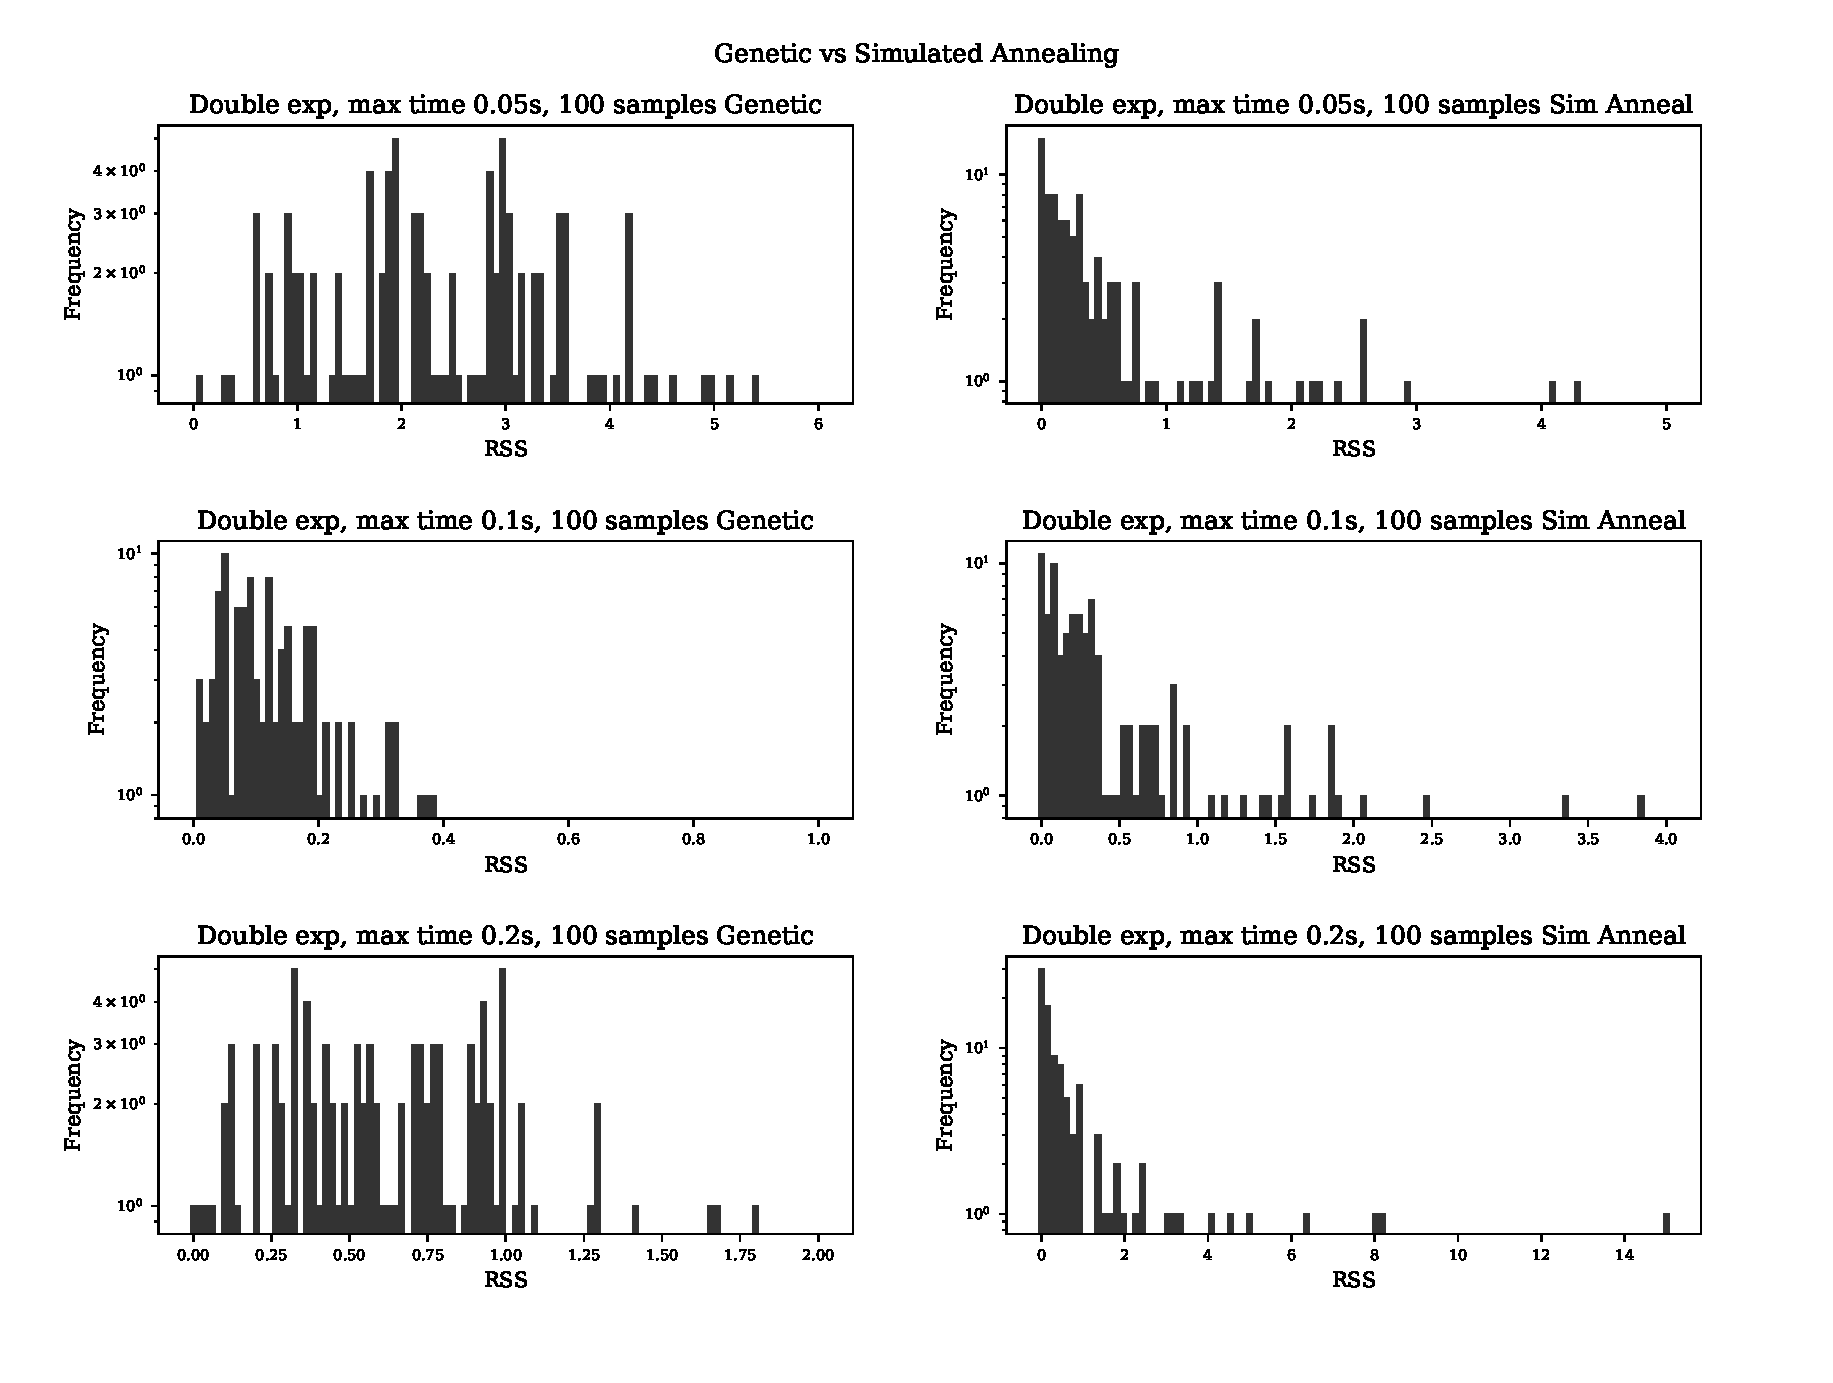
\includegraphics[width=15.0cm]{appendix/sim_anneal_genetic/pop_512/plot_name_11.eps}
    \captionsetup{font={it}}
    \caption{Genetic Algorithm Population Size 512 vs Simulated Annealing}
    \label{fig:ga_vs_sim_512_3}
  \end{center}
\end{figure}






